\documentclass[twocolumn]{article}

\usepackage{listings}
\usepackage{graphicx}

\title{Lab#3\\Computational Physics I - Phys381}
\author{Guilherme Contesini , 10140201 }

%%%%%%%%%%%%%%%%%%%%%%%%%%%%%%%%%%%%%%%%%%%%%%%%%%%%%%%%%%%%%%%%%%%%%%%%%%%%%%%%%%%%%%%%%%%%%%%%%%%%%%%%%%%%%%%%%%%%%%%%

\begin{document}
\maketitle
\date

%%%%%%%%%%%%%%%%%%%%%%%%%%%%%%%%%%%%%%%%%%%%%%%%%%%%%%%%%%%%%%%%%%%%%%%%%%%%%%%%%%%%%%%%%%%%%%%%%%%%%%%%%%%%%%%%%%%%%%%%

\section{Part-1}
\paragraph*{}
In part 1 we will build several matrices that contains only '0' and '1', the position inside the matrix where those numbers appear will be chosen by a random number. The law will be if the random number if less or equal to a probability of transition that place inside the matrix will receive a '0', if the random number is greater than this probability of transition this place will receive number '1'.

\newpage
\begin{figure}[h!]
\begin{center}
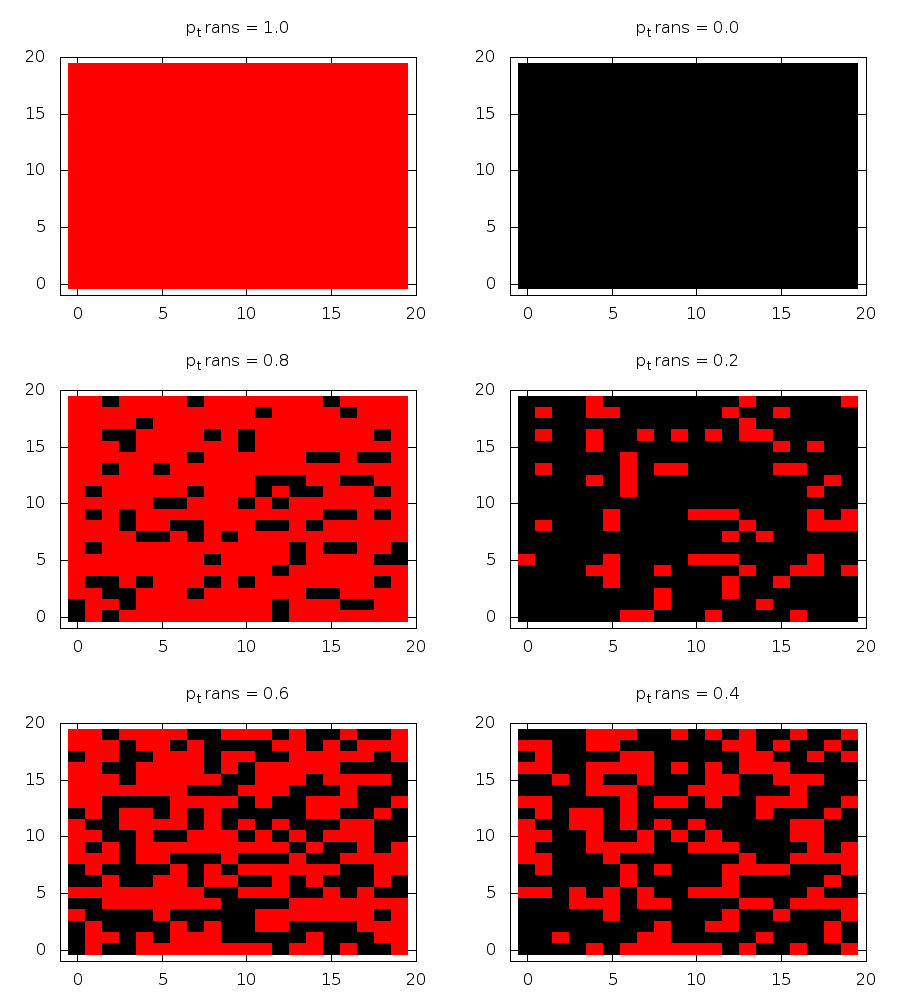
\includegraphics[width=3in]{contesini-figure1.png}
\caption{Color map Matrix}
\label{Color map Matrix}
\end{center}
\end{figure}

\newpage
\section{Part-2}



\begin{figure}[h!]
\begin{center}
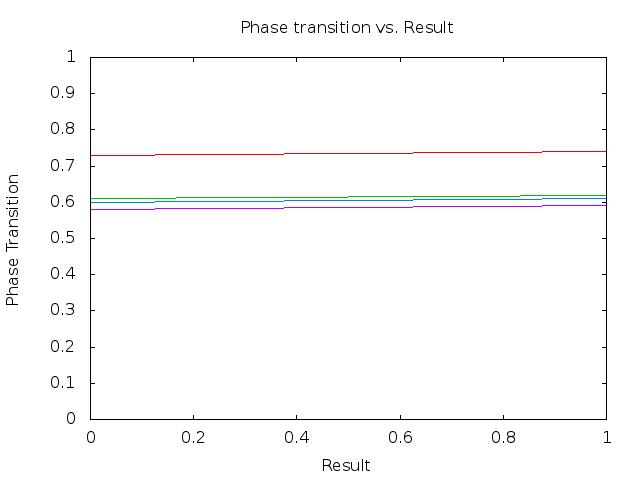
\includegraphics[width=3in]{contesini-figure2.png}
\caption{Color map Matrix}
\label{Color map Matrix}
\end{center}
\end{figure}

\section{Codes & Scripts}

\subsection{fortran code}
\begin{verbatim}
program guilhermecontesinigrid

  implicit none
  integer :: true_int ,
 false_int , size_int, count_int
  real :: p_trans

  open(12,file="savedgrid.txt
",action="write")
  true_int = 1
  false_int= 0
  p_trans = 0.00

  write(6,*), "Type the size of
 your square matrix:" 
  read(*,*) size_int

  do count_int=0,100
     call buildgrid( true_int ,
false_int,size_int,p_trans )
     p_trans = p_trans + 0.01
  enddo

  close(12)
end program


subroutine buildgrid( true_int 
, false_int , size_int , p_trans )

  integer, intent(in) :: true_int
 , false_int , size_int
  real, intent(in) :: p_trans
  integer , allocatable ,
 dimension(:,:) :: mygrid_int
  integer :: i , j
  real :: rand 

  allocate(mygrid_int
(size_int,size_int))
  call random_seed()

  do i=1,size_int
    do j=1,size_int

      call random_number(rand)
      
      if(rand < p_trans) then
        mygrid_int(i,j)
 = true_int
      else
        mygrid_int(i,j)
 = false_int
      endif
    end do
  end do
  call savegrid( size_int 
, p_trans , mygrid_int )
  deallocate(mygrid_int)

end subroutine



subroutine savegrid( size_int
 , p_trans ,mygrid_int )

  integer, intent(in) :: 
size_int 
  integer, dimension(size_int
  ,size_int)
 :: mygrid_int
  real, intent(in) ::  p_trans
  integer :: i , j
  
  do i=1,size_int
     do j=1,size_int
        if(j == size_int)
 then 
           write(12,"(i1)",
advance='yes') mygrid_int(i,j)
        else
           write(12,"(i1,1x)",
advance='no') mygrid_int(i,j)
        end if
        !write(12,"(f3.1)",
advance='yes') p_trans
     end do
  end do
  write(12,"(f3.1)",
advance='yes') p_trans
end subroutine


\end{verbatim}

\subsection{gnuplot script - 1}
\begin{verbatim}
reset
set terminal png
set output 'matrix.png'
set palette maxcolor 2
unset colorbox
set palette defined 
(0 'black', 1 'red')
set multiplot

set size 0.4,0.4

set origin 0.5,0.8
set title 'p_trans = 0.0'
plot 'savedgrid.txt' 
matrix with image notitle
set origin 0.5,0.4
set title 'p_trans = 0.2'
plot 'savedgrid.txt' 
matrix with image notitle
set origin 0.5,0.0
set title 'p_trans = 0.4'
plot 'savedgrid.txt'
 matrix with image notitle
set origin 0.0,0.0
set title 'p_trans = 0.6'
plot 'savedgrid.txt' 
matrix with image notitle
set origin 0.0,0.4
set title 'p_trans = 0.8'
plot 'savedgrid.txt' 
matrix with image notitle
set origin 0.0,0.8
set title 'p_trans = 1.0'
plot 'savedgrid.txt'
 matrix with image notitle

reset
\end{verbatim}


\subsection{gnuplot script - 1}
\begin{verbatim}
program guilhermecontesinigrid

  implicit none
  integer :: true_int , 
  false_int , size_int, count_int,
   result
   , loop_size
  integer , allocatable , 
  dimension(:,:) :: mygrid_int
  real :: p_trans

   p_trans = 0.00

  open(12,file="transitiondata.txt"
  ,action="write")

  do loop_size=10,150,10
    size_int= loop_size

    do count_int = 0 ,100
      allocate(mygrid_int(size_int
      ,size_int))
      call buildgrid( true_int ,
      false_int,size_int,p_trans ,
      mygrid_int)
      if(size_int==10 .or. size_int==50
       .or. size_int==100 .or. 
       size_int==150 )then
      
        call phasetransitioncheck
        (mygrid_int,size_int,
        size_int,result)
        write(12,*)size_int,
        p_trans,result
      
      endif
      p_trans = p_trans + 0.01
      deallocate(mygrid_int)
    enddo

    write(12,*)
    write(12,*)
    p_trans=0.00  
  enddo
  close(12)

contains

subroutine buildgrid( true_int 
, false_int , size_int , p_trans 
,mygrid_int )

  integer, intent(in) :: size_int
  real, intent(in) :: p_trans
  integer :: true_int , false_int , i , j
  integer, dimension(size_int
  ,size_int) :: mygrid_int
  real :: rand 

  true_int = 1
  false_int= 0


  call random_seed()

  do i=1,size_int
    do j=1,size_int
      call random_number(rand)
      if(rand .le. p_trans) then
        mygrid_int(i,j) = true_int
      else
        mygrid_int(i,j) = false_int
      endif
    end do
  end do

end subroutine

subroutine savegrid( size_int
 ,mygrid_int )

  integer, intent(in) :: size_int
  integer, dimension(size_int,
  size_int) :: mygrid_int
  integer :: i , j
  
  do i=1,size_int
     do j=1,size_int
        if(j == size_int) then 
           write(12,"(i1)",
           advance='yes') mygrid_int(i,j)
        else
           write(12,"(i1,1x)",
           advance='no') mygrid_int(i,j)
        end if
     end do
  end do
  write(12,'(1x)',advance='yes')
  write(12,'(1x)',advance='yes')
end subroutine

end program

subroutine phasetransition
check(grid,m,n,outcome)
implicit none
integer :: i
integer, intent(in) :: n, m
integer, intent(inout), 
dimension(m,n) :: grid
integer, intent(out) :: outcome 
logical :: success, q

outcome = 0
success = .false.
do i=1, m
q = ScanMatrix(grid, i)
success = success .or. q
end do

outcome = outcome + merge(1, 0, 
success)

contains

logical function ScanMatrix(grid,
 start)
integer, dimension(m,n), intent
(inout) :: grid
integer, intent(in) :: start
ScanMatrix = CheckSpanning(grid, 
1, start, int(start+1,1))
end function ScanMatrix

recursive function CheckSpanning
(grid, i, j, k) result(through)

logical :: through
integer, dimension(m,n), intent
(inout) :: grid
integer, intent(in) :: i, j
integer(kind=1), intent(in) :: k
logical, dimension(4) :: q
through = .false.
if (i < 1) return
if (m < i) return
if (j < 1) return
if (n < j) return
if (1_1 /= grid(i, j)) return
grid(i, j) = k
q(1) = CheckSpanning(grid,i+0,j+1,k)
q(2) = CheckSpanning(grid,i+0,j-1,k)
q(3) = CheckSpanning(grid,i+1,j+0,k)
q(4) = CheckSpanning(grid,i-1,j+0,k)
through = (i == m) .or. any(q)
end function CheckSpanning

end subroutine phasetransitioncheck
\end{verbatim}
%%%%%%%%%%%%%%%%%%%%%%%%%%%%%%%%%%%%%%%%%%%%%%%%%%%%%%%%%%%%%%%%%%%%%%%%%%%%%%%%%%%%%%%%%%%%%%%%%%%%%%%%%%%%%%%%%%%%%%%%
\section{Conclusion :}
\paragraph*{}

%%%%%%%%%%%%%%%%%%%%%%%%%%%%%%%%%%%%%%%%%%%%%%%%%%%%%%%%%%%%%%%%%%%%%%%%%%%%%%%%%%%%%%%%%%%%%%%%%%%%%%%%%%%%%%%%%%%%%%%%
\end{document}